\setchapterstyle{kao}
\setchapterpreamble[u]{\margintoc}

\chapter{Detecting Low Energetic Double Cascades}
\labch{double_cascade_performance}


\section{Reconstruction}

\subsection{Table-Based Minimum Likelihood Algorithms}

\subsection{Double Cascade Hypothesis}

\subsection{Modification to Low Energy Events}

\section{Cross Checks}
\subsection{Simplistic Sets}

After generation the events are processed with standard Photon, Detector, L1, and L2 processing and then Taupede+MuMillipede is run on top of the L2 files. Multiple versions with different parameters were produced, some with the OscNext baseline parameters, some without detector noise (in Det level) and some with h2-50cm holeice model, to match the holeice model that was used to generate the photonics tables.


\paragraph{BrightDom Cleaning}

To investigate the effect of the BrightDom cleaning cut the 194601 set without detector noise (and baseline hole ice model) is used. The BrightDom cleaning is needed to stop a few DOMs with many photon hits to drive the reconstruction because this leads to large biases in the energy estimations. Historically, the BrightDom cleaning was removing all DOMs that had a charge larger than 10 times the mean charge. After quickly checking some charge distributions and how the mean behaves it was clear that the cut should better be defined based on a metric that is less affected by outliers, like the median. \reffig{bright_dom_cleaning_charges_mean_median} shows where the mean and the median are located for an example event. The cut was re-defined to use the median instead of the mean and 10\% of the simulation were processed with \href{https://github.com/LeanderFischer/I3_HNL_Decay/blob/a6838ec48e0a2d4f6547cbe064d2928ec55fb76d/submission_scripts/process/process_Taupede.py}{Taupede} using 30x and 100x the median as BrightDom cutoff. \reffig{bright_dom_cleaning_charges_median_scales} shows where these values fall for the same example event.

% \begin{figure}[h!]
%     \subfloat[\labfig{bright_dom_cleaning_charges_mean_median}]{
%         \includegraphics[width=.45\linewidth]{figures/upgoing_string_81_gen_level/brightdom_cleaning/median_and_mean_L2_00001.i3.zst_SplitInIcePulses_frame_0.png}
%         }
%     \subfloat[\labfig{bright_dom_cleaning_charges_median_scales}]{
%         \includegraphics[width=.45\linewidth]{figures/upgoing_string_81_gen_level/brightdom_cleaning/median_scales_L2_00001.i3.zst_SplitInIcePulses_frame_0.png}
%         }
%     \caption{Charge distribution of example event showing mean and median charge (left) and different scales of median charge (right).}
%     \labfig{bright_dom_cleaning_charges}
% \end{figure}

As a quick check of the performance of both cuts the decay length resolution/bias and the resolutions/biases of all energies were checked. The reconstructed decay length is almost not affected by applying this cut, which is as expected, because it is mostly dependent on the arrival time of the photons. The effect on the reconstructed energy is much stronger, where a looser cut (100x) shows a significantly larger bias than the tighter cut at (30x). Even though this was not a highly sophisticated optimization of the BrightDom cut, an improvement was achieved by changing from mean to median and selecting the tighter cut (of the two tested). It's hard to tell how this would perform for high energy events, but I'm quite certain that a definition based on the median would be more reliable than on the mean.

% \begin{figure}[h!]
%     \subfloat[\labfig{bright_dom_cleaning_performance_decay_length_bias}]{
%         \includegraphics[width=.45\linewidth]{figures/upgoing_string_81_gen_level/brightdom_cleaning/median_decay_length_bias_fullset_larger_range_unweighted.png}
%         }
%     \subfloat[\labfig{bright_dom_cleaning_performance_total_energy_bias}]{
%         \includegraphics[width=.45\linewidth]{figures/upgoing_string_81_gen_level/brightdom_cleaning/compare_bright_dom_cuts_fractional_reco_total_energy_error_fully.png}
%         }
%     \caption{Decay length bias (left) and total energy bias (right).}
%     \labfig{bright_dom_cleaning_performance}
% \end{figure}

\section{Performance}

\subsection{Energy/Decay Length Resolution}

\todo{describe the "good fit" selection}

\subsubsection{2-D Histograms}

\textbf{Things to mention about the 2d-hists:}
\begin{itemize}
    \item total energy resolution looks very good, above \SI{10}{\gev} it's almost unbiased and the 1-sigma resolution band is below \SI{20}{\percent}
    \item individual cascade resolutions mirror this behavior, but are starting to stabilize in energy at lower energies around \SIrange{5}{6}{\gev} with a broader resolution band of \SI{50}{\percent}, but reducing drastically with increasing energy (down to \SI{20}{\percent} at \SI{100}{\gev})
    \item interestingly, the second cascade energy reconstruction performs slightly worse, although they have the same energy ranges. This could hint at an asymmetry in the reconstruction process (might relate to how the two cascades are parameterized) or be due to the different positions and the dominantly up-going direction used in the sampling combined with the DOMs looking down (relate this to the sampling distribuitons explained/shown in the previous chapter)
    \item the decay length resolution looks much worse. In the region between \SIrange[range-phrase={~and~}]{20}{80}{\meter} it's roughly unbiased, but 1-sigma resolution band is quite wide with a lot of outliers towards short reconstructed lengths. Below \SI{20}{\meter} the reconstructed lengths are always over-estimating the true and above \SI{80}{\meter} a population of events start to dominate where the decay lengths isn't getting reconstructed at all, which might indicate that one of the cascades wasn't observers. (Relate to the fact that this marginalizes over all energies, meaning also all events which have one cascade with very low energy are included here.)
    \item another interesting feature is the band of reconstructed lengths around \SI{100}{\meter}, which is probabaly related to the spacing between most of the strings, which favors the reconstruction to be around this value, because that's the distance at which light can be observed, just from the fact that the DOMs are spaced at this distance (for low energetic cascades, this can dominate the reconstruction)
\end{itemize}


\begin{figure*}[h]
	\centering
    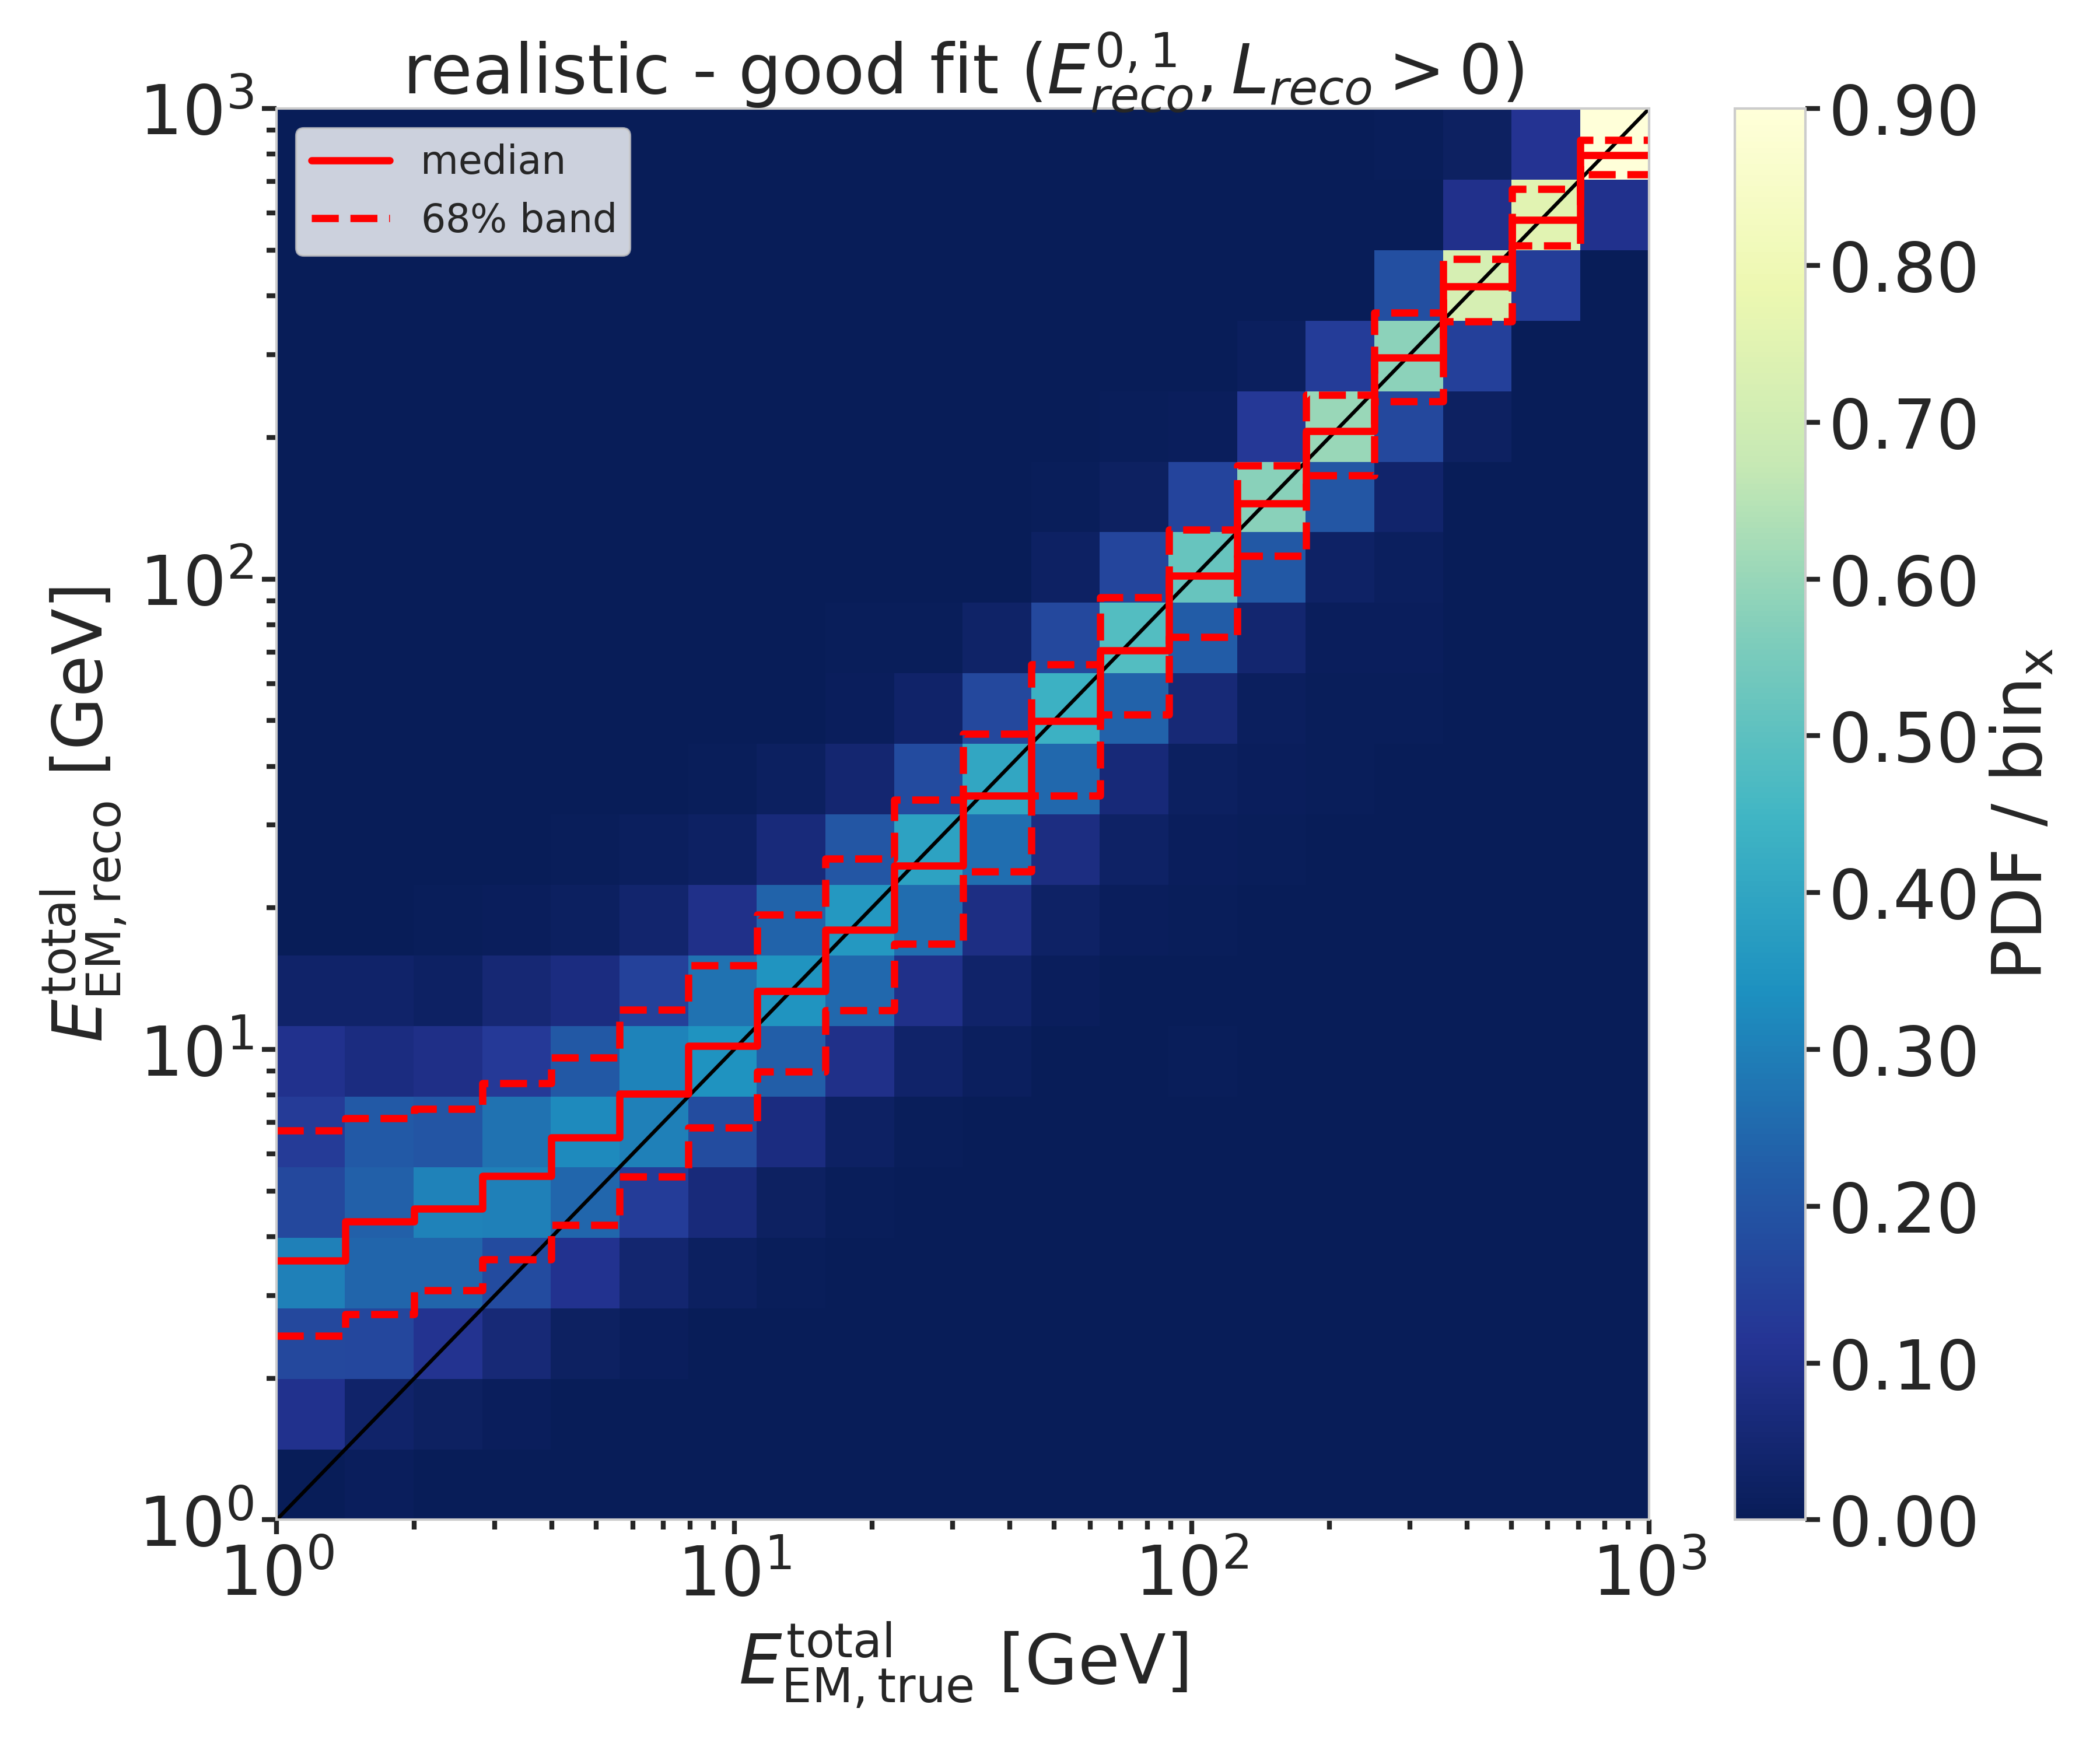
\includegraphics[width=0.49\linewidth]{figures/model_independent_simulation/results/realistic/2d_hists/194603_reco_total_energy_vs_true_total_energy_goodfit_step_contours.png}
    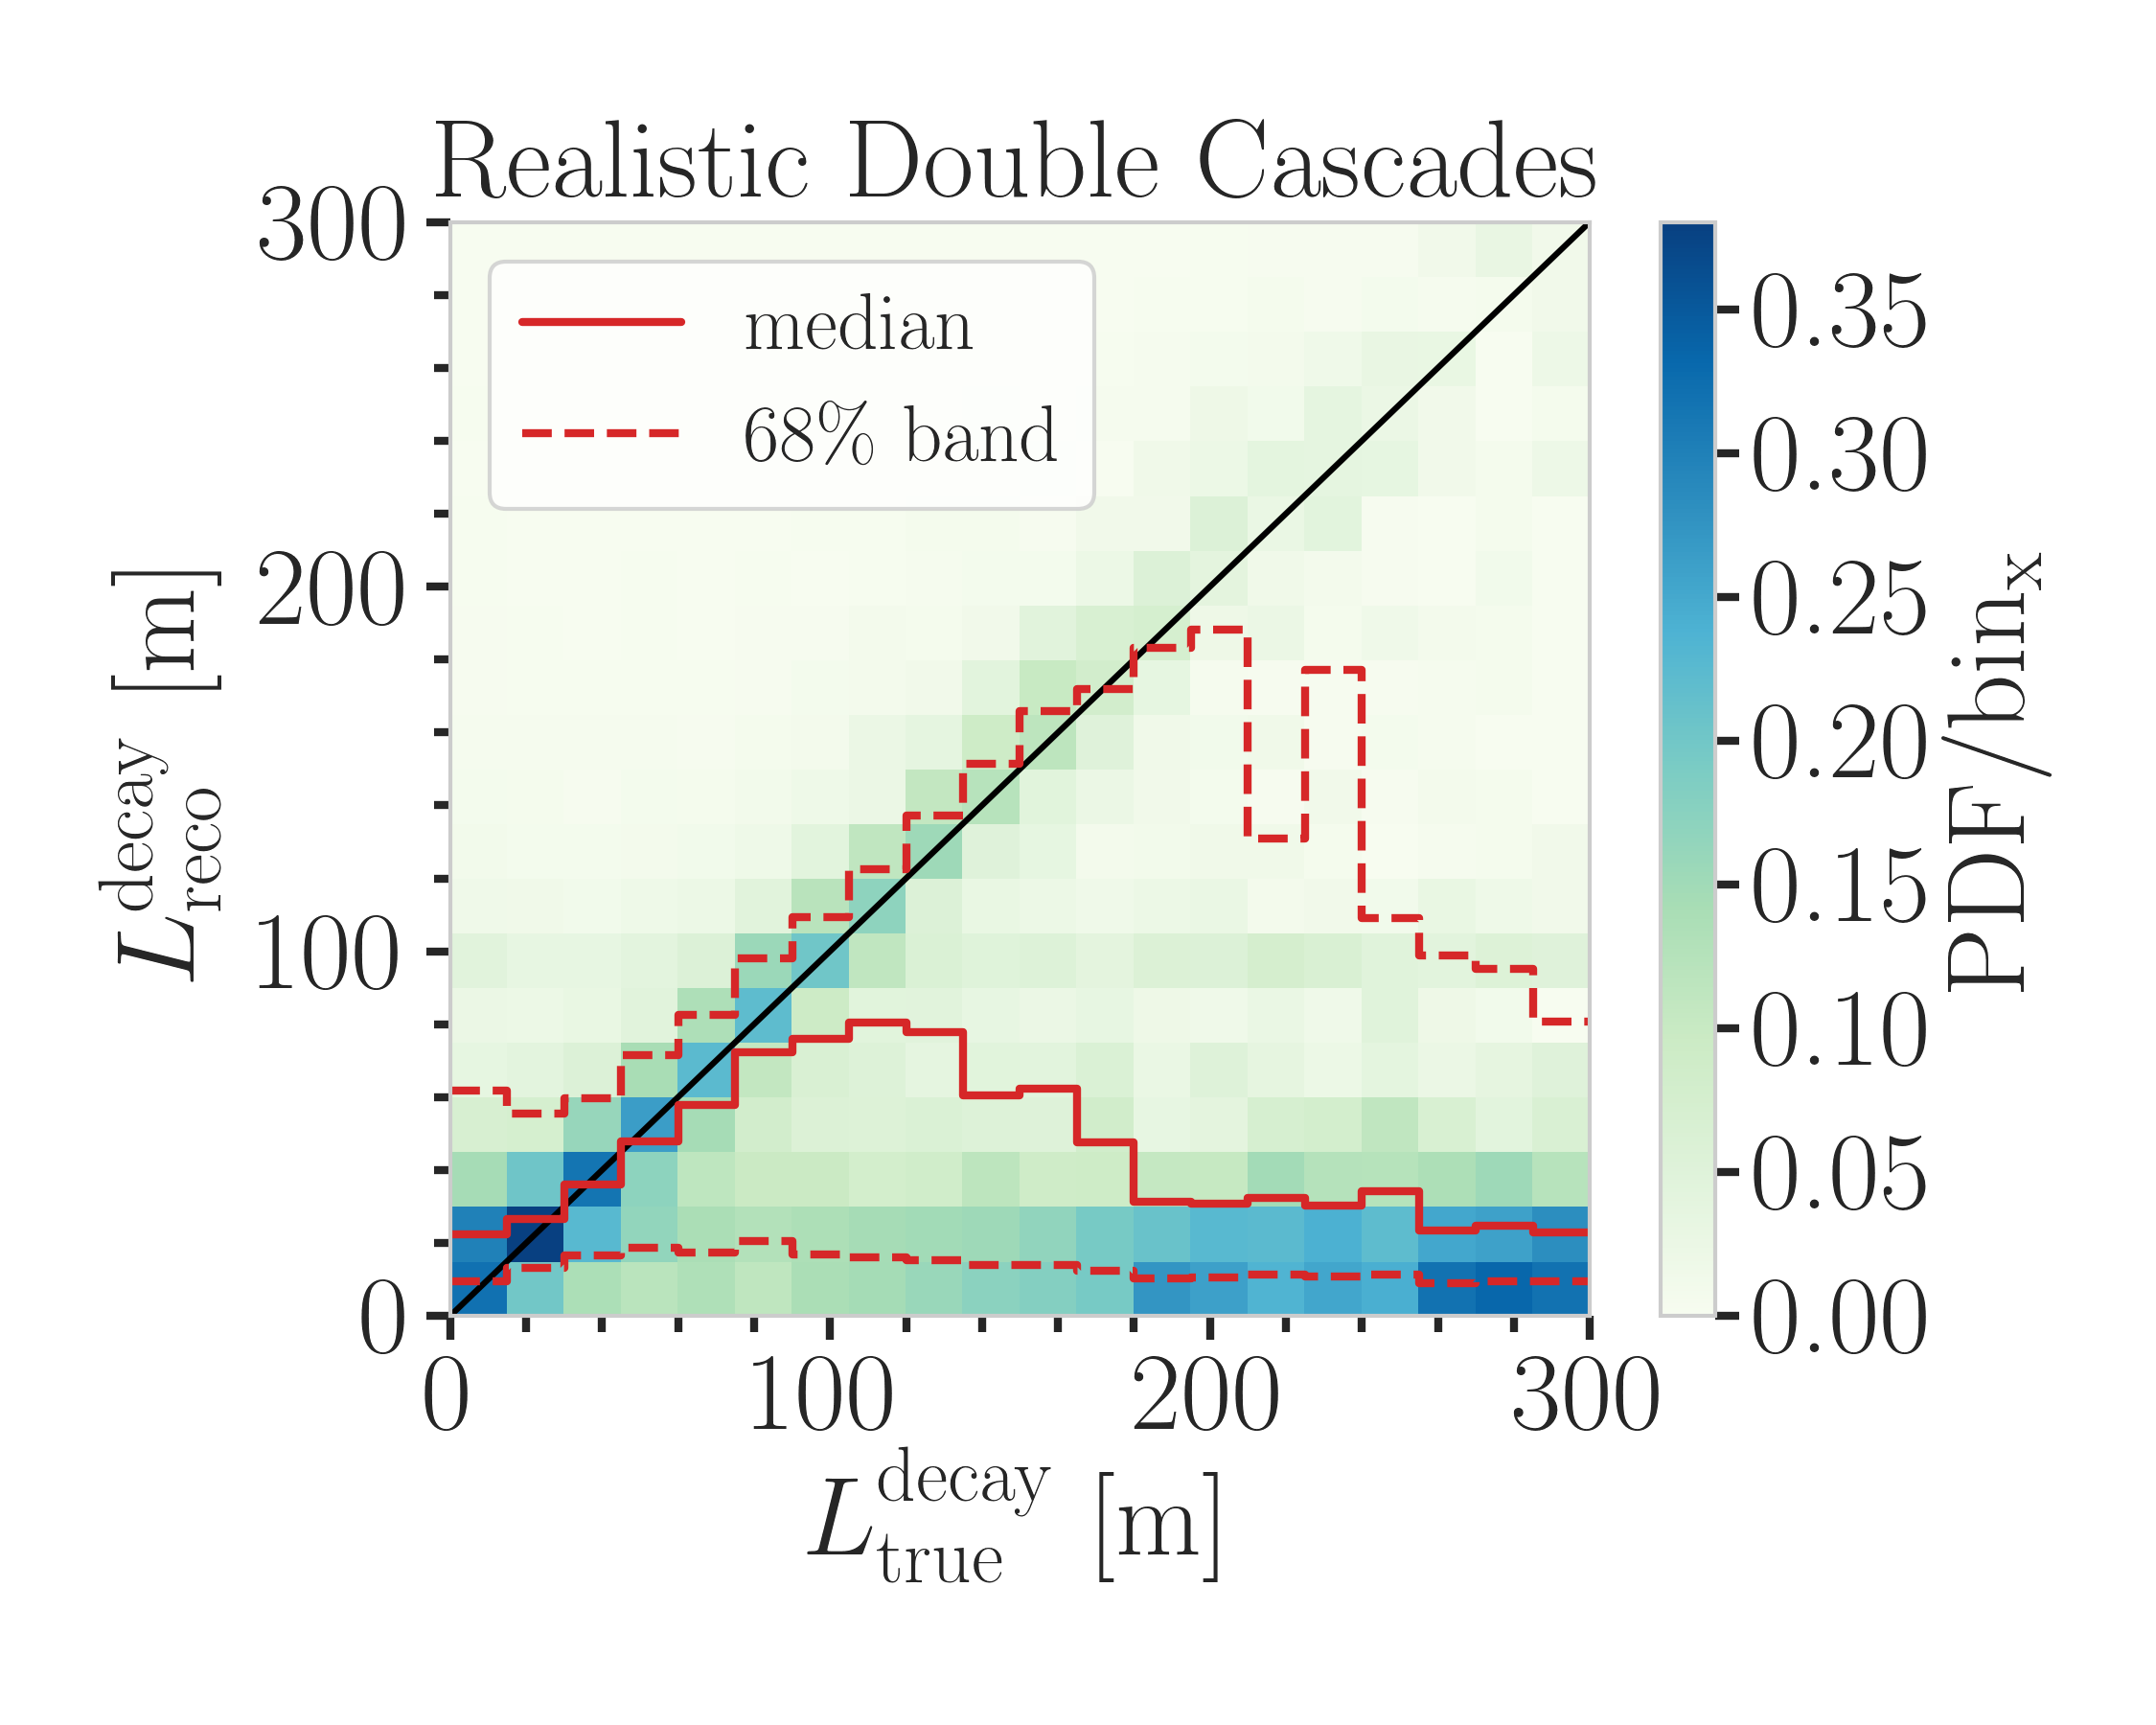
\includegraphics[width=0.49\linewidth]{figures/model_independent_simulation/results/realistic/2d_hists/194603_reco_decay_length_vs_true_decay_length_goodfit_step_contours.png}
    \caption[]{}
    \labfig{total_energy_decay_length_2dhists}
\end{figure*}

\begin{figure*}[h]
	\centering
    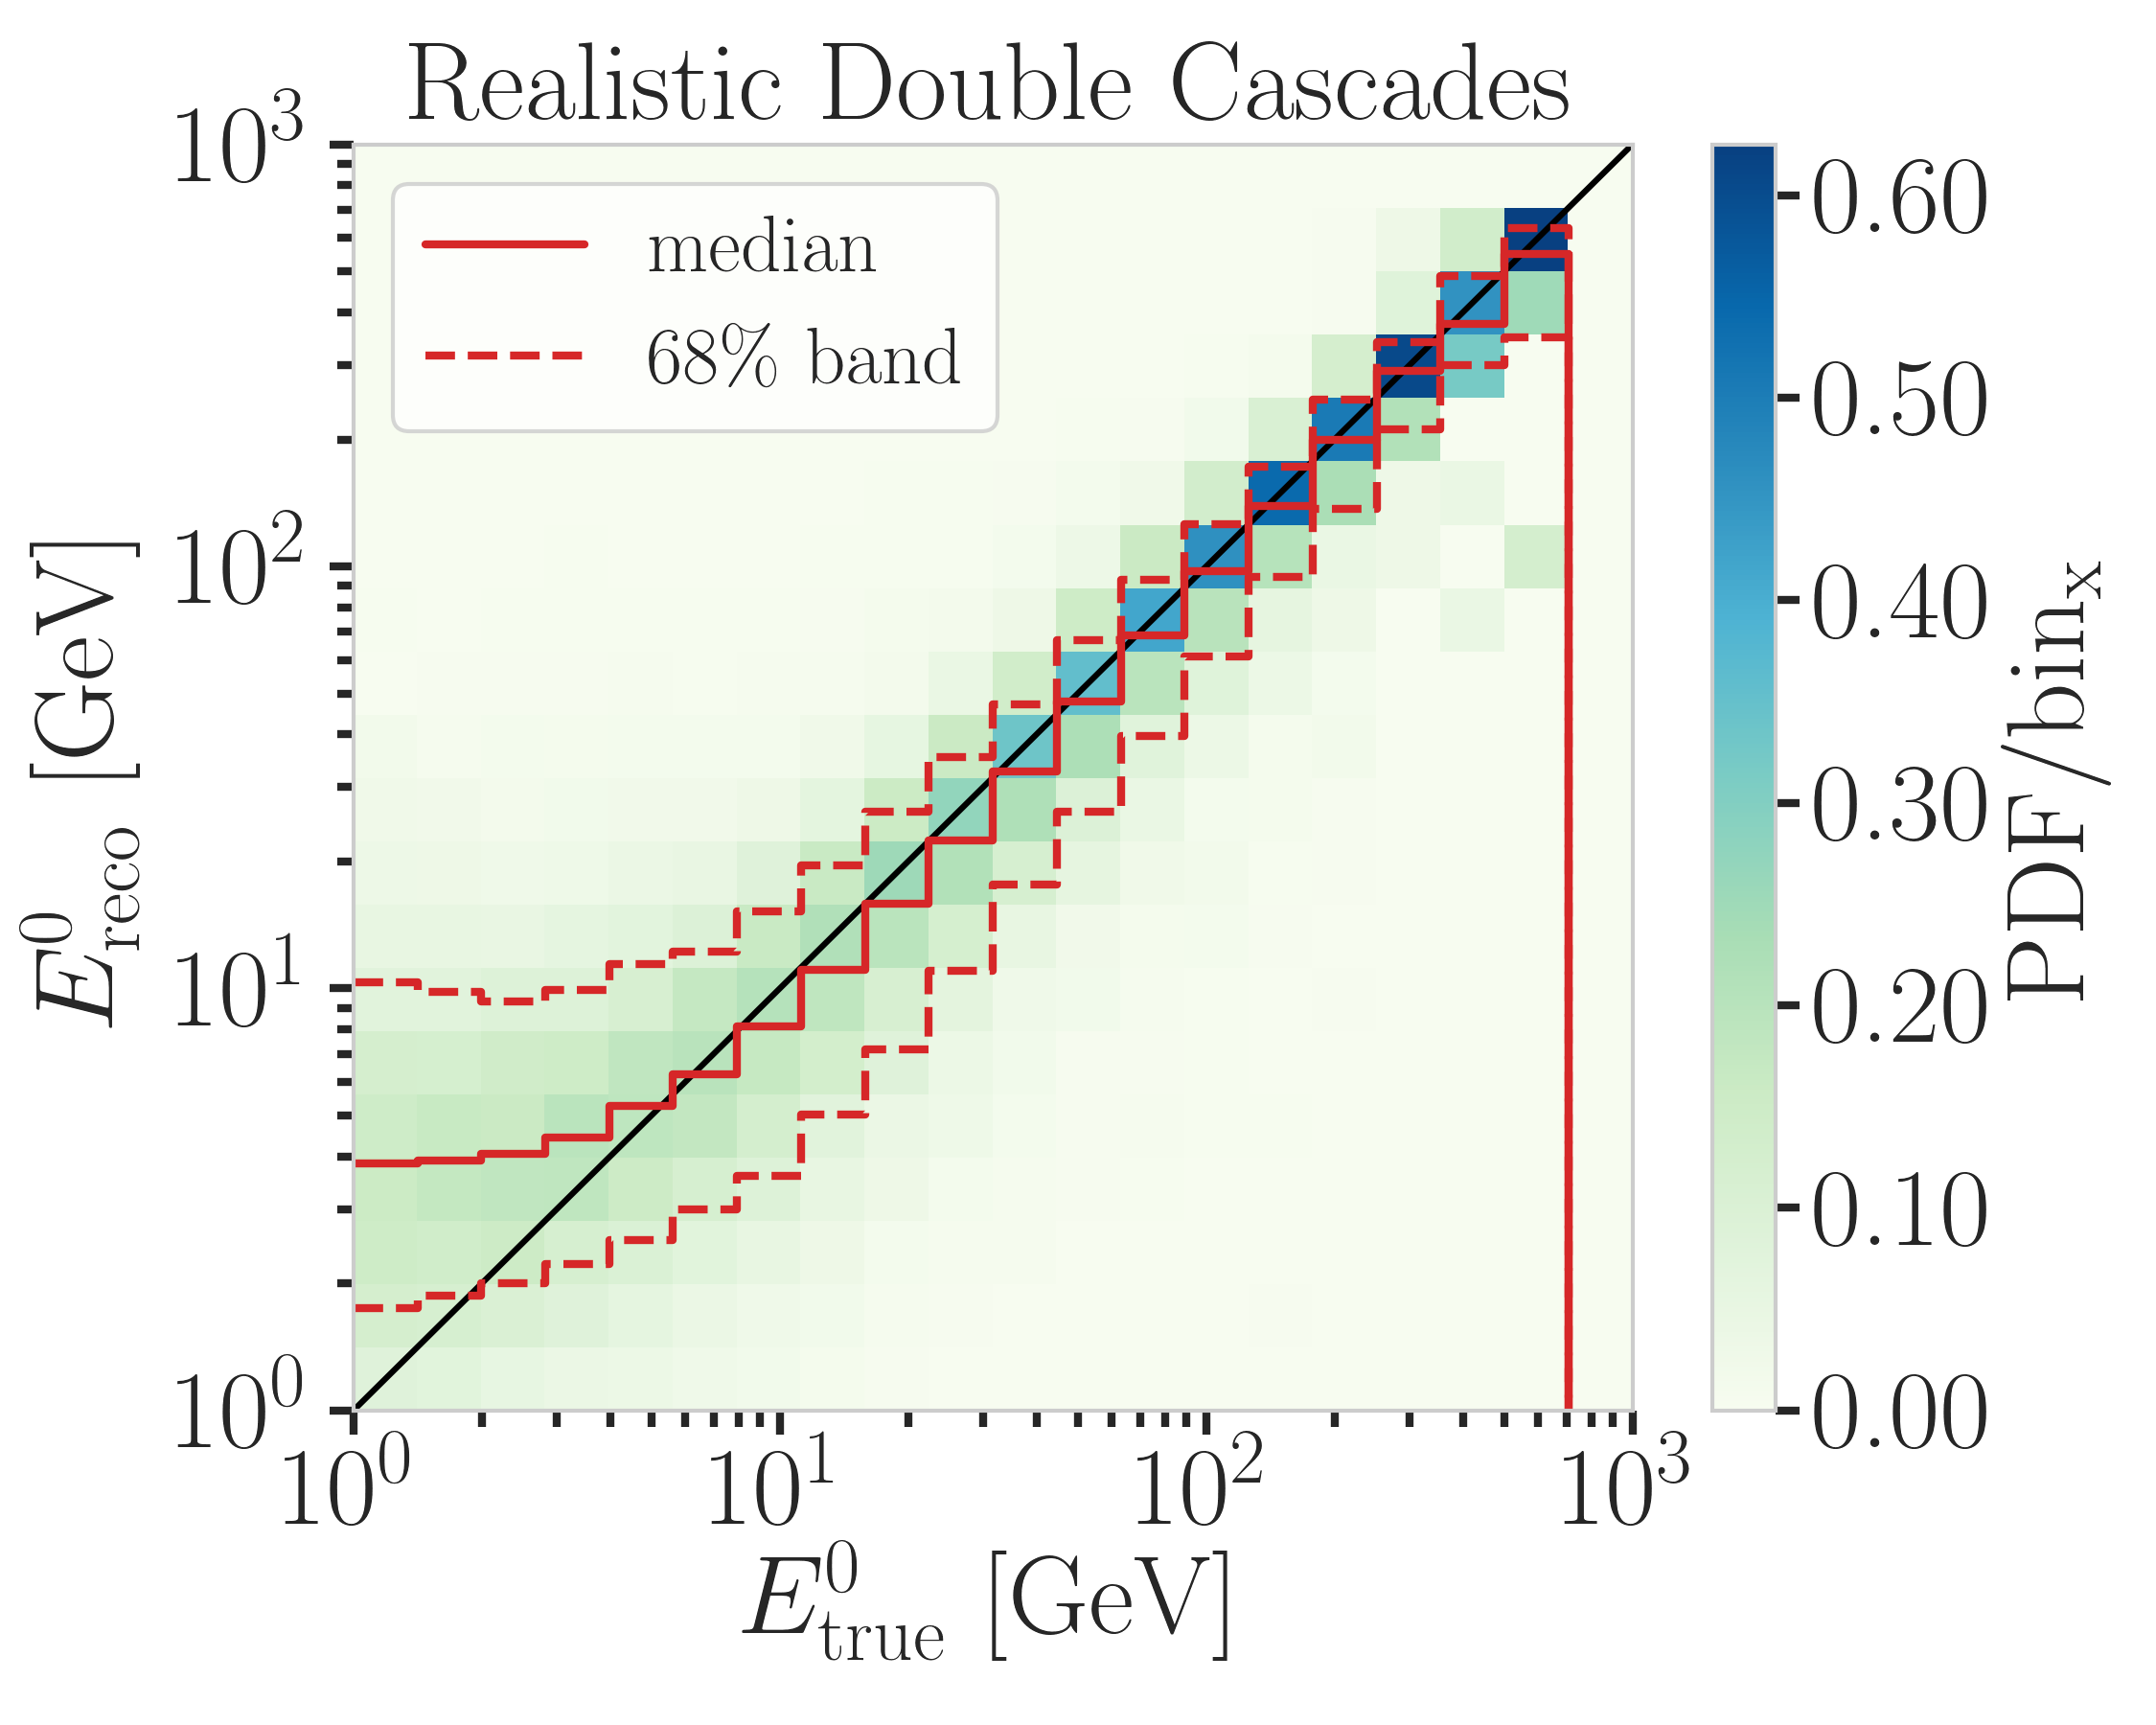
\includegraphics[width=0.49\linewidth]{figures/model_independent_simulation/results/realistic/2d_hists/194603_casc0_reco_energy_vs_casc0_true_energy_goodfit_step_contours.png}
    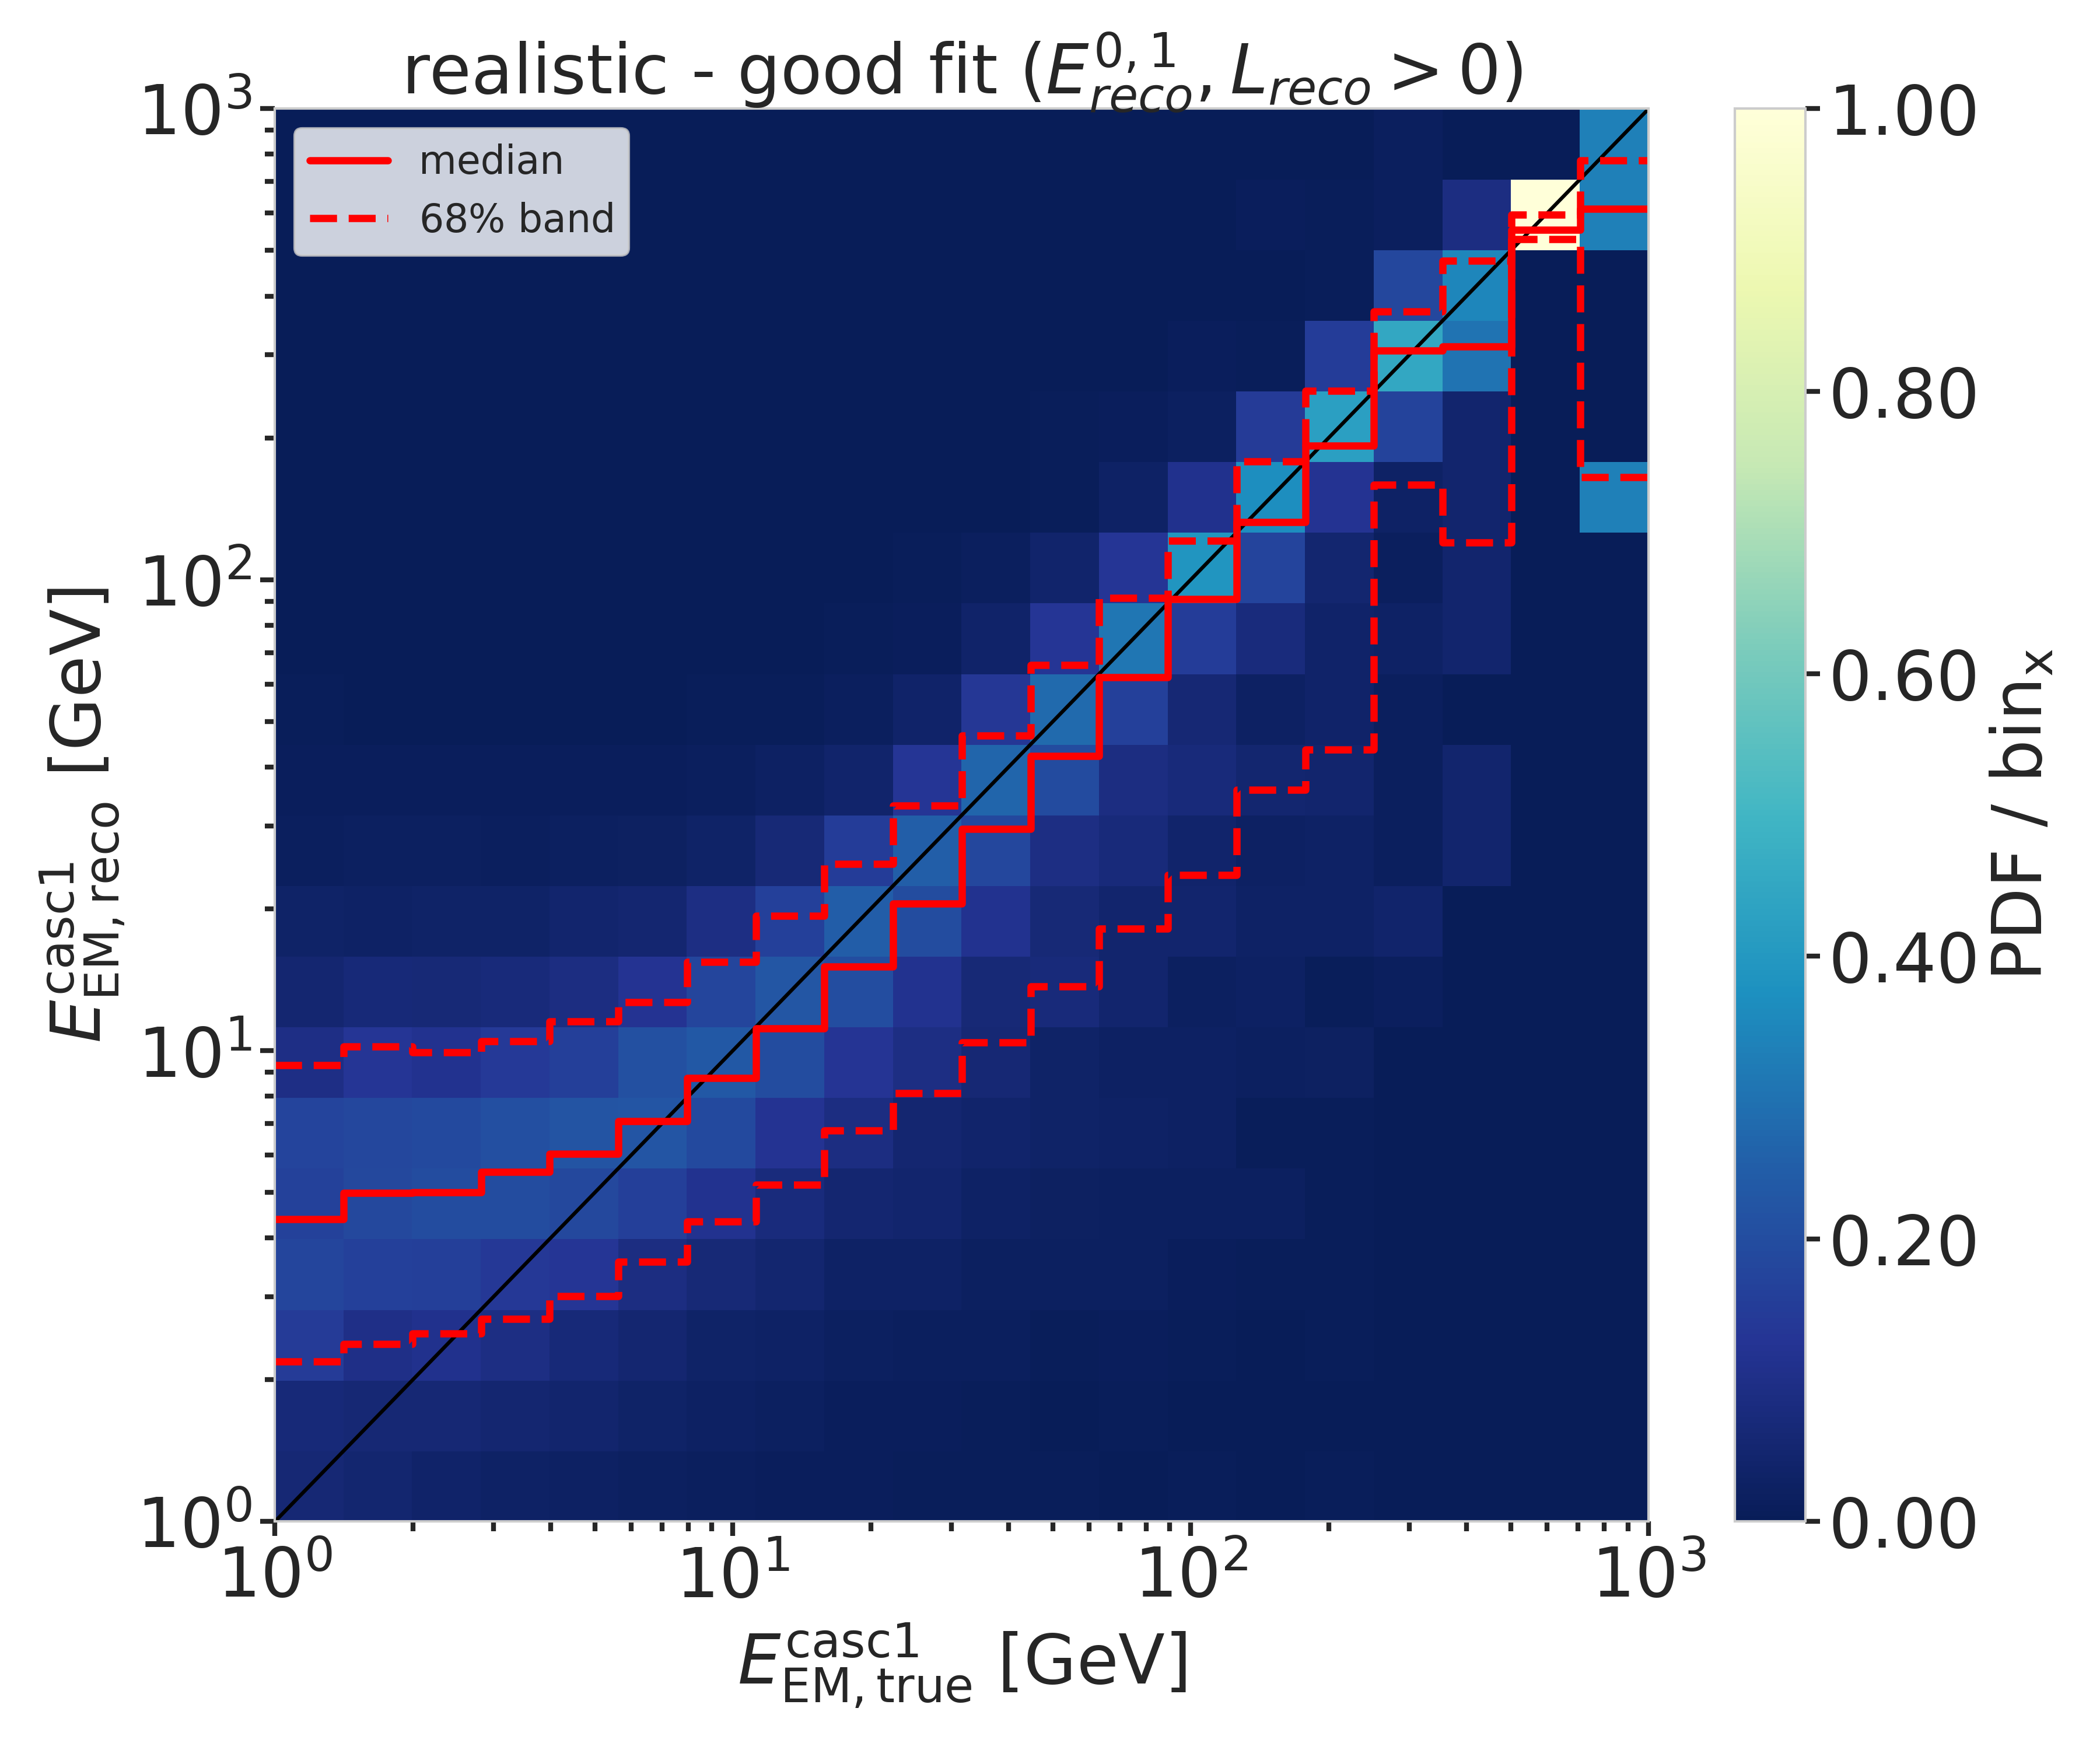
\includegraphics[width=0.49\linewidth]{figures/model_independent_simulation/results/realistic/2d_hists/194603_casc1_reco_energy_vs_casc1_true_energy_goodfit_step_contours.png}
    \caption[]{}
    \labfig{cascade_energy_2dhists}
\end{figure*}


\subsubsection{Energy Resolution}

\textbf{Things to mention about the energy resolution:}
\begin{itemize}
    \item Here it can be seen more clearly how the median total energy resolution starts to stabilize around 0.0 at \SI{10}{\gev}, while for lower energies the reconstruction is over-estimating the true energy. This is a known behavior of energy reconstructions in IceCube, which is mainly due to a selection effect. Only events with a certain amount of light can be reconstructed, which means that the ones with true small energies that are still in the sample are events with over average light production due to fluctuations or other effects?
\end{itemize}

\begin{figure}[h]
	\centering
    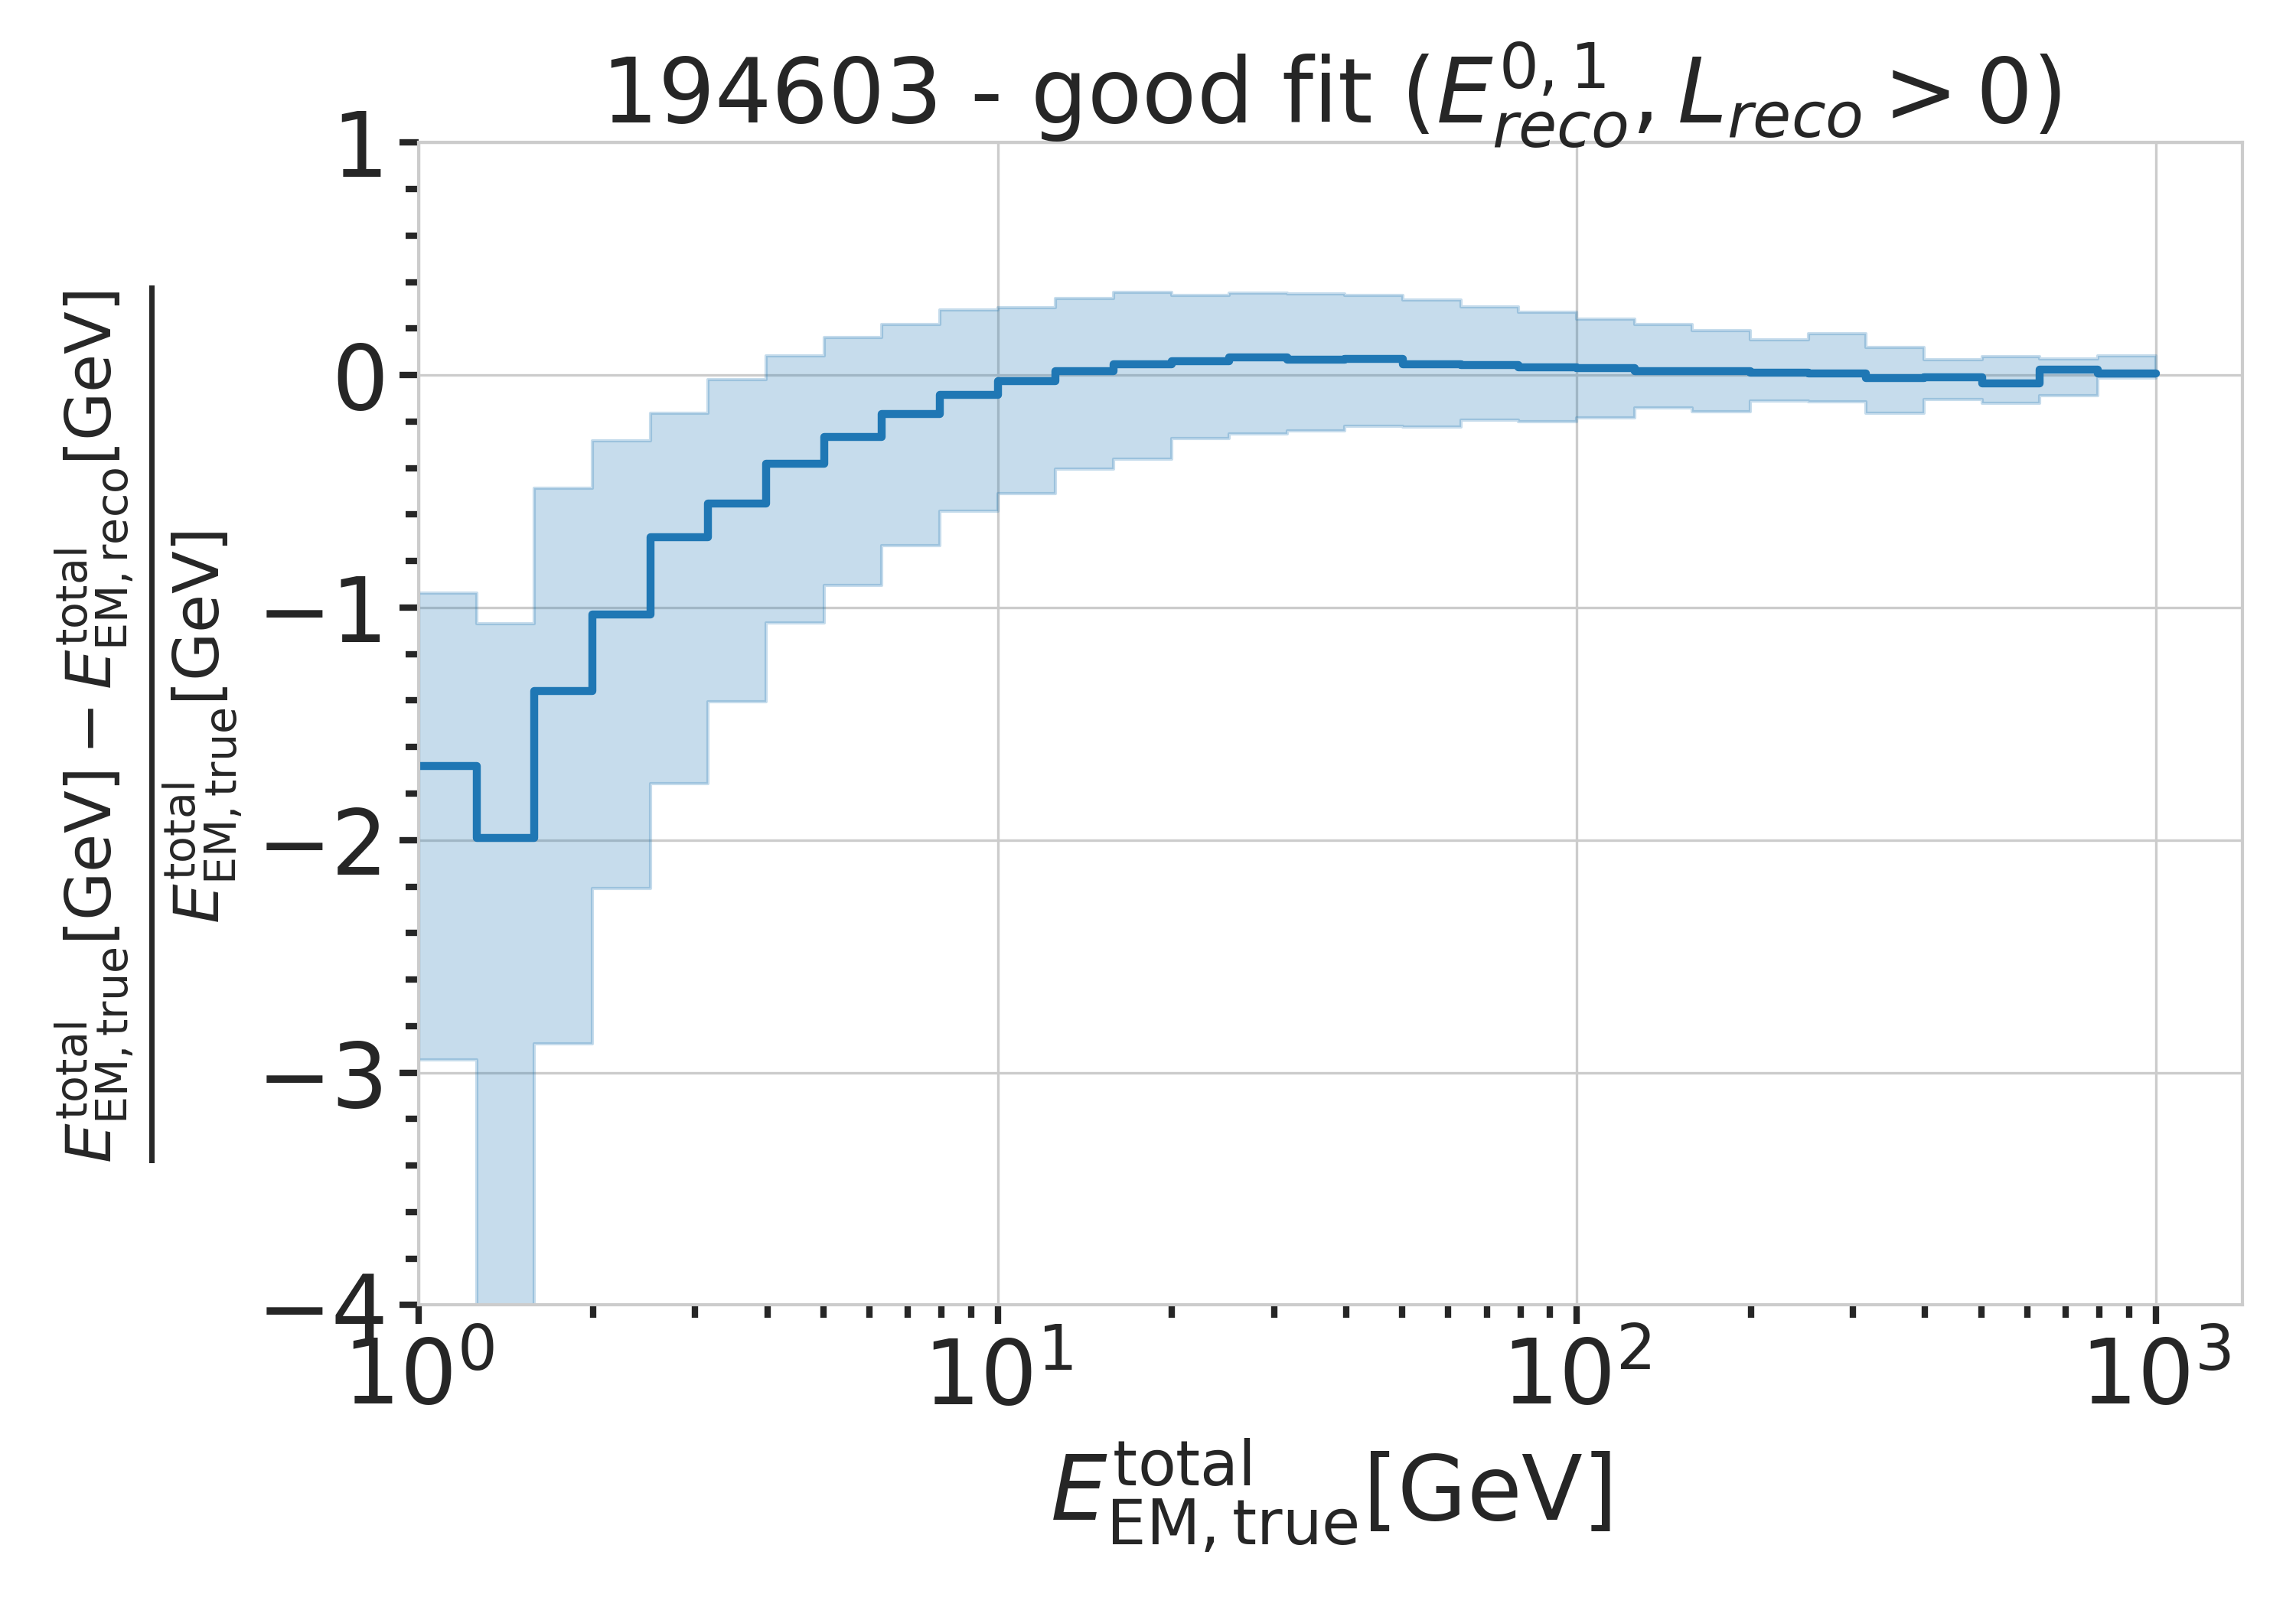
\includegraphics{figures/model_independent_simulation/results/realistic/resolutions/194603_fractional_reco_total_energy_error_goodfit.png}
    \caption[]{}
    \labfig{total_energy_bias_vs_energy}
\end{figure}


\subsubsection{Decay Length Resolution}

\textbf{Things to mention about the decay length resolution:}
\begin{itemize}
    \item As already mentioned before, the decay length resolution is much worse than the energy resolutions. \reffig{decay_length_bias_vs_length} also shows that the median is below 0.0 for short true length and above 0.0 and approaching 1.0 for long true lengths.
    \item To investigate whether this is really due to the fact that one of the cascades is not observed, the decay length resolution was plotted against the total energy of the event and the minimum energy of the two cascades \reffig{decay_length_bias_vs_energies}.
    \item It can be seen that the median of the decay length resolution stabilizes at 0.0 for a total energy above \SI{20}{\gev}, but the spread of the distribution is still quite large with a 1-sigma band of \SIrange{80}{100}{\percent}.
    \item From the plot against the minimum energy it can be seen that the decay length resolution starts to be unbiased for a minimum energy of the cascades of \SI{7}{\gev}, with an equivalently large spread.
    \item A preliminary takeaway from this is that the decay length reconstruction is not reliable at all for events with a total energy below \SI{20}{\gev} or a minimum cascade energy below \SI{7}{\gev}.
\end{itemize}

\begin{figure}[h]
	\centering
    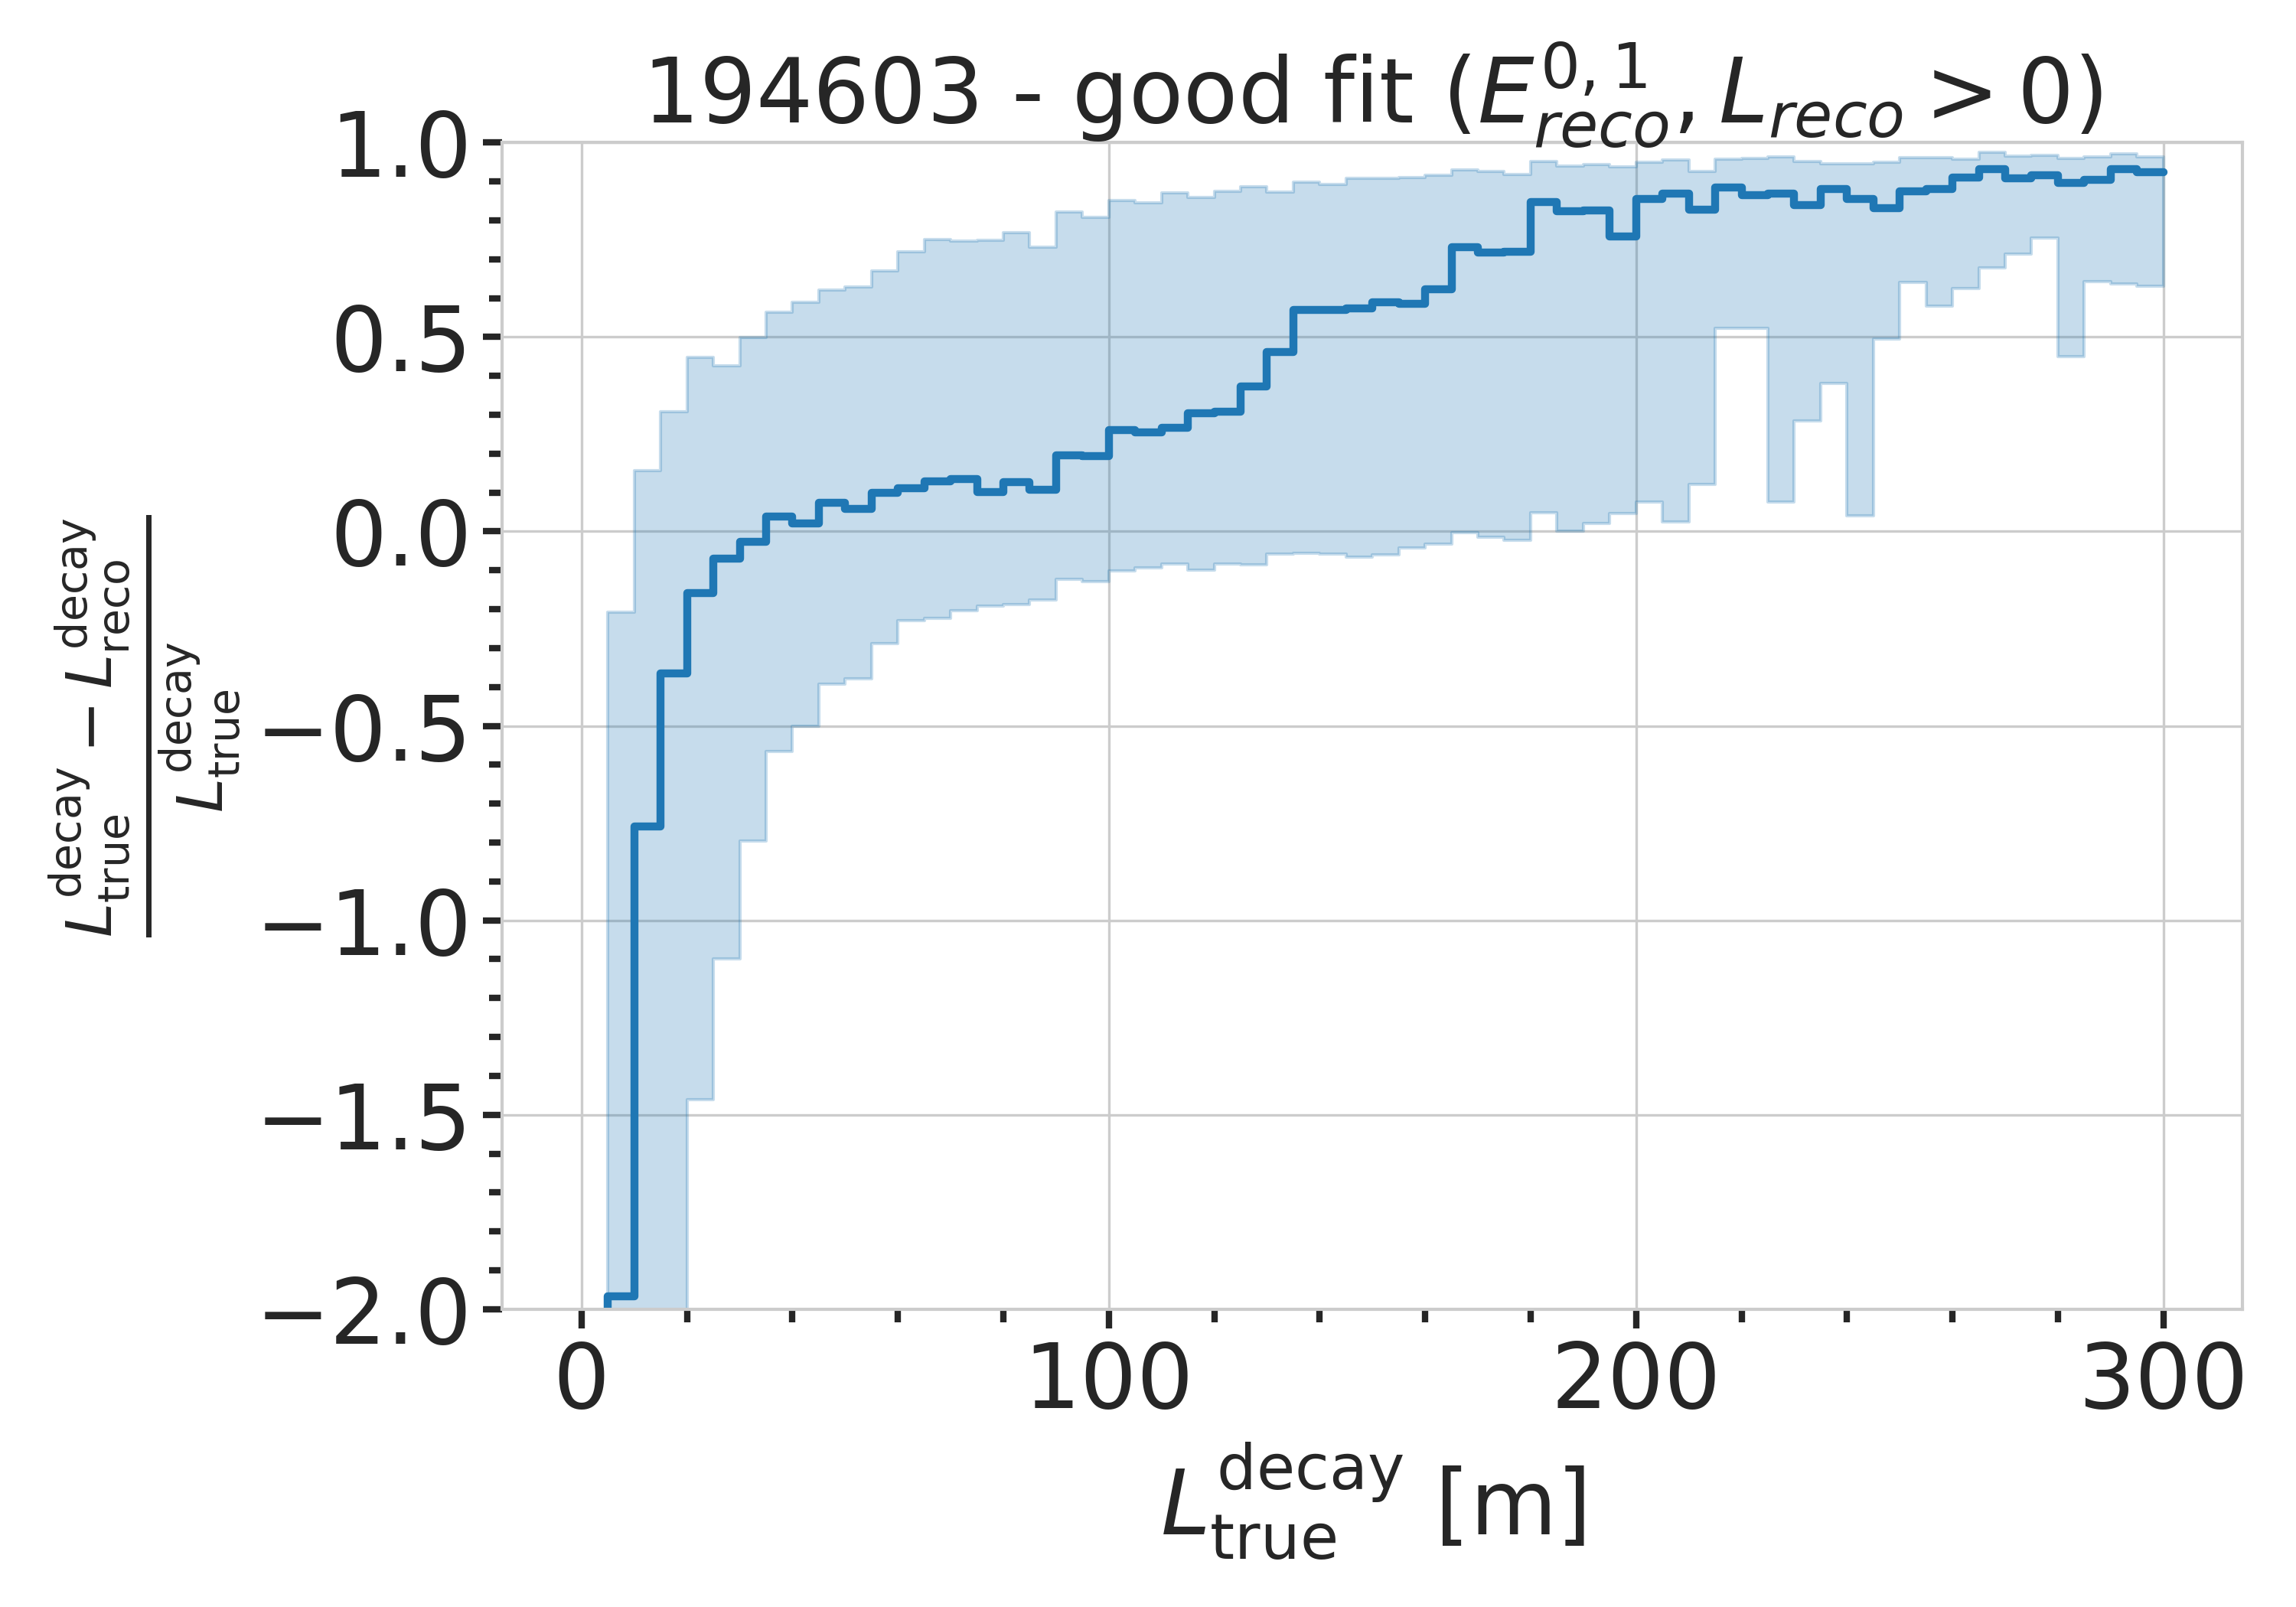
\includegraphics{figures/model_independent_simulation/results/realistic/resolutions/194603_median_decay_length_bias_goodfit_log_unweighted.png}
    \caption[]{}
    \labfig{decay_length_bias_vs_length}
\end{figure}


\begin{figure*}[h]
	\centering
    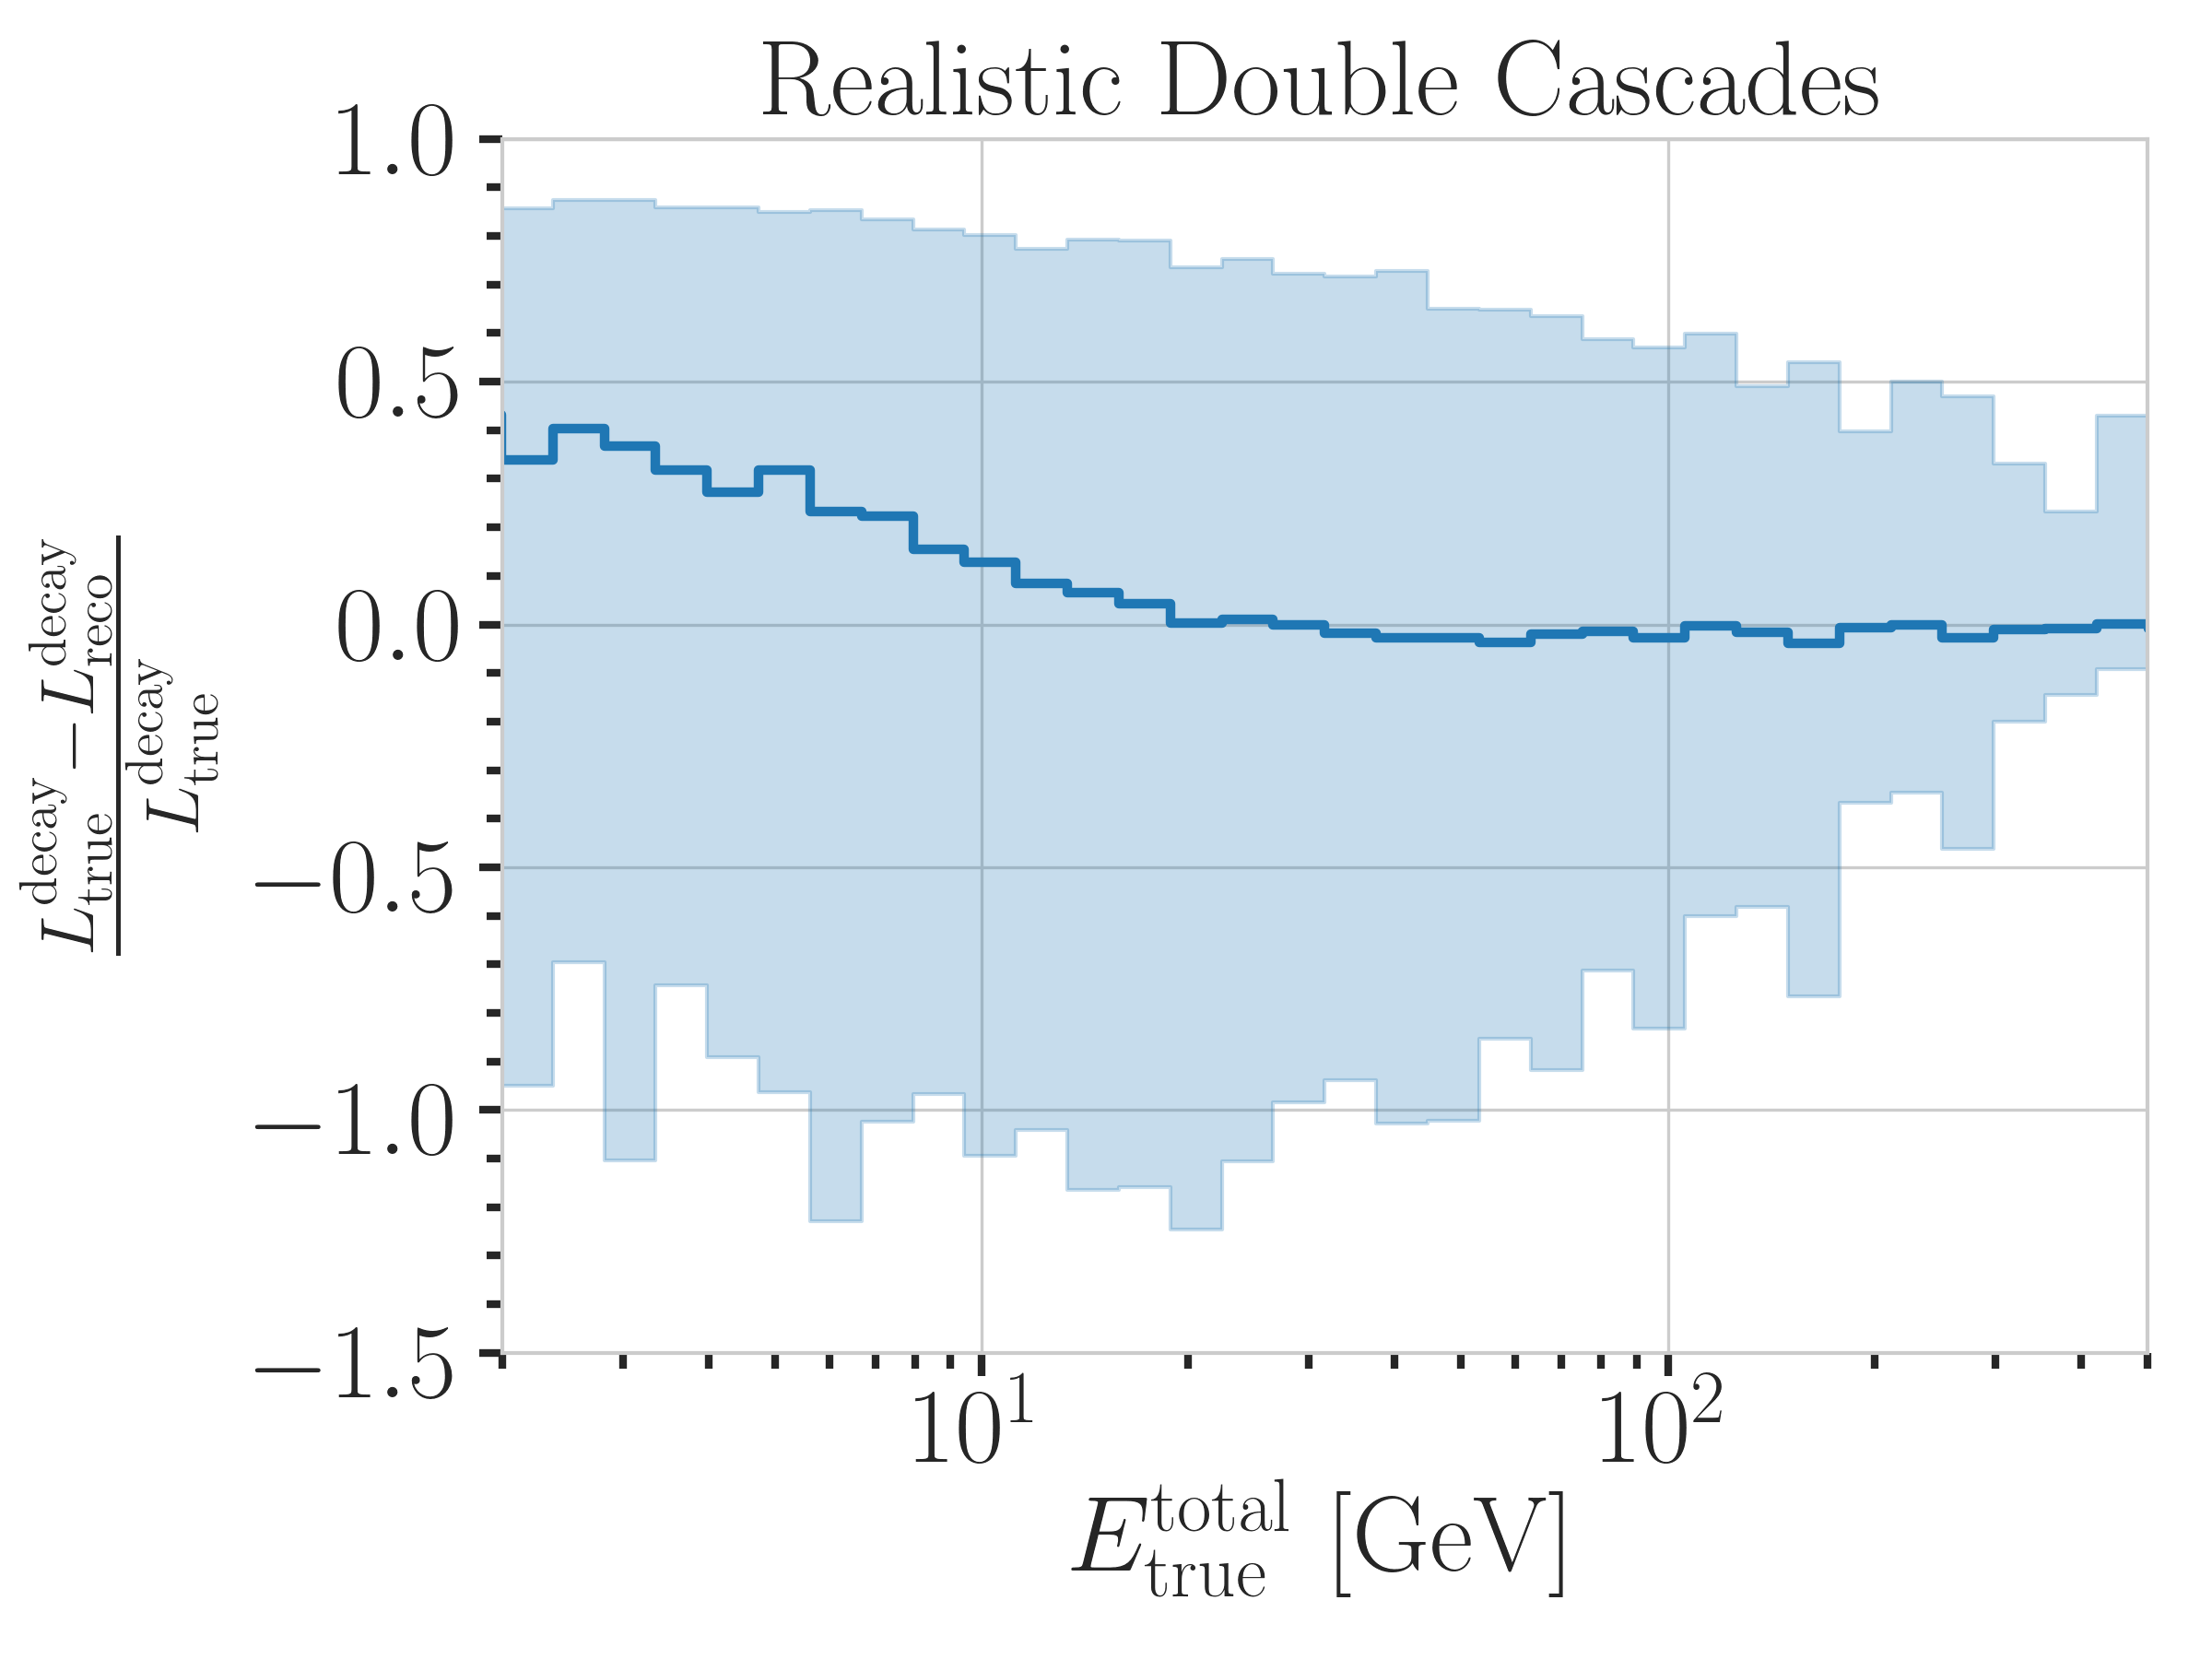
\includegraphics[width=0.49\linewidth]{figures/model_independent_simulation/results/realistic/resolutions/194603_median_decay_length_bias_vs_tot_energy_goodfit_log_unweighted.png}
    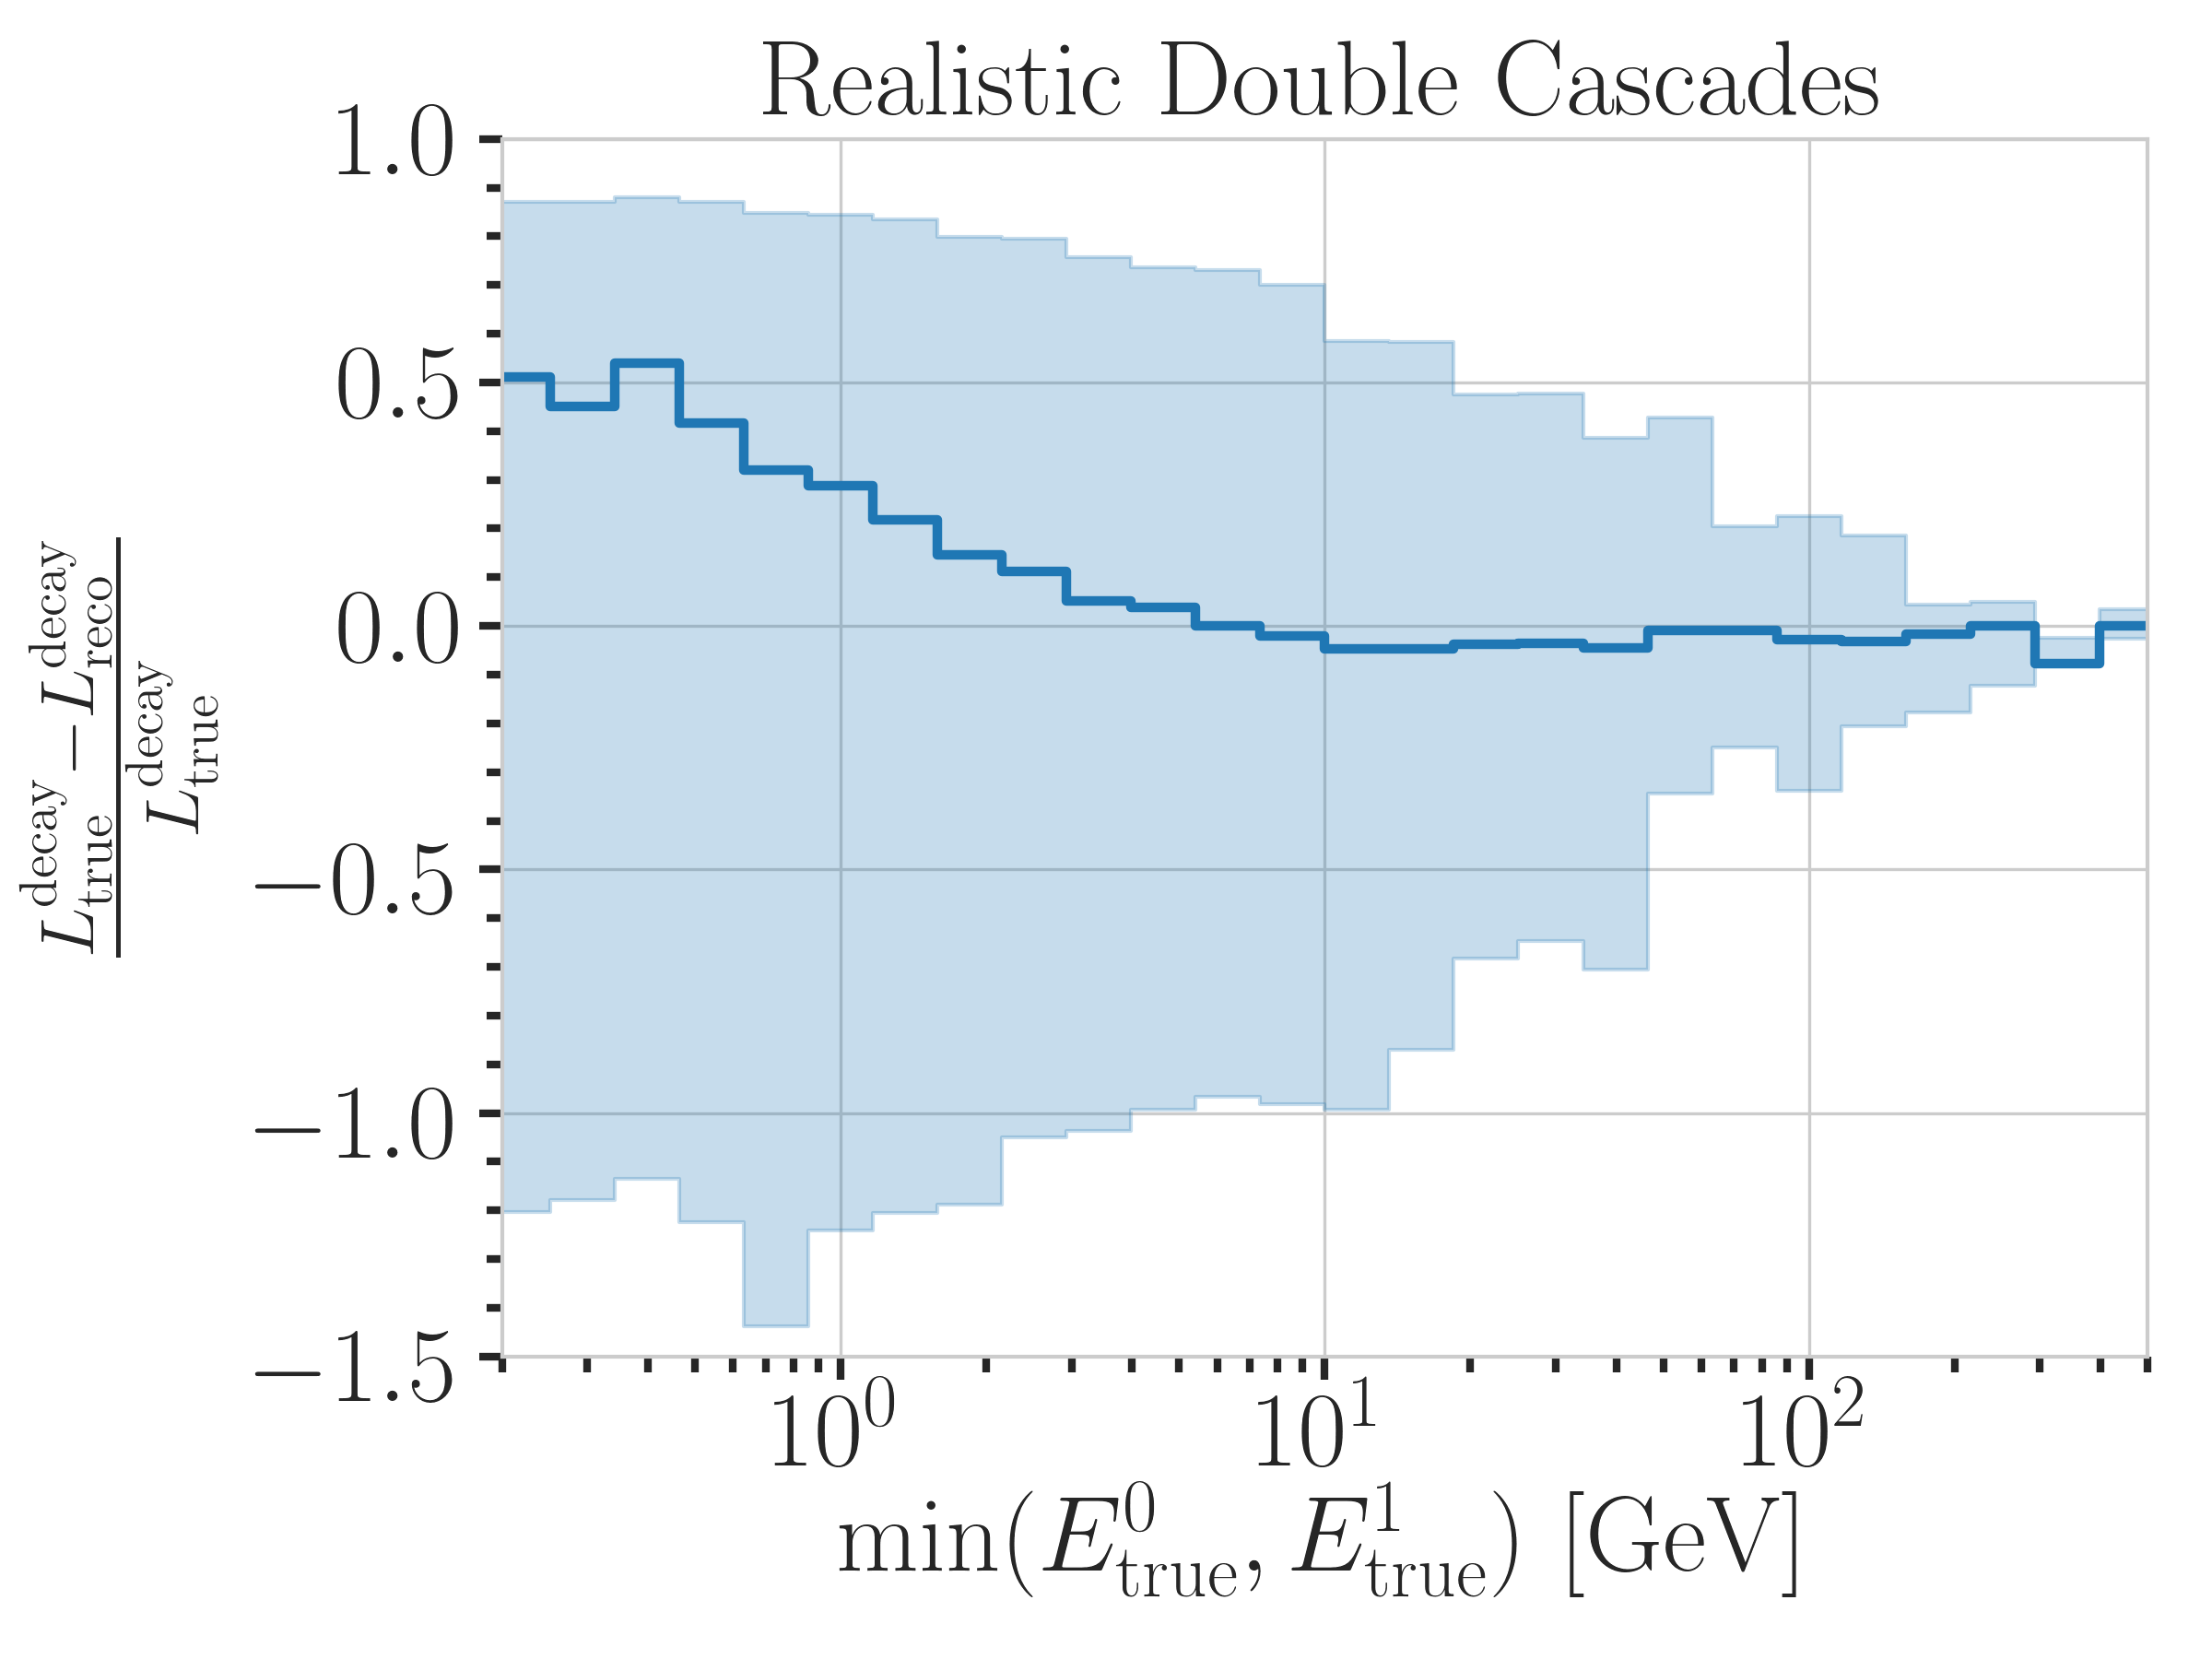
\includegraphics[width=0.49\linewidth]{figures/model_independent_simulation/results/realistic/resolutions/194603_median_decay_length_bias_vs_min_energy_goodfit_log_unweighted.png} 
    \caption[]{}
    \labfig{decay_length_bias_vs_energies}
\end{figure*}


\subsection{Double Cascade Classification}


% \begin{figure}
%     \includegraphics{xx}
%     \caption[]{}
%     \labfig{xx}
% \end{figure}



